%%%%%%%%%%%%%%%%%%%%%%%%%%%%%%%%%%%%%%%%%%%%%%%%%%%%%%%%%%%%%%%%%%%%%%%%%%%%%%%%
%
% Examples of graphs generated with pgfplots.
% Copyright (C) 2014  Joshua Ellis
%
% This program is free software; you can redistribute it and/or modify it under
% the terms of the GNU General Public License as published by the Free Software
% Foundation; either version 2 of the License, or (at your option) any later
% version.
%
% This program is distributed in the hope that it will be useful, but WITHOUT ANY
% WARRANTY; without even the implied warranty of MERCHANTABILITY or FITNESS FOR A
% PARTICULAR PURPOSE.  See the GNU General Public License for more details.
%
% You should have received a copy of the GNU General Public License along with
% this program; if not, write to the Free Software Foundation, Inc., 51 Franklin
% Street, Fifth Floor, Boston, MA 02110-1301 USA.
%
%%%%%%%%%%%%%%%%%%%%%%%%%%%%%%%%%%%%%%%%%%%%%%%%%%%%%%%%%%%%%%%%%%%%%%%%%%%%%%%%
\documentclass[tikz]{standalone}

\usepackage{pgfplots}
\pgfplotsset{compat=1.10}

% Use externalization so that we do not have to generate all the graphs every
% single time.  All the generated figures are stored in the "pgf-img" directory.
%
% The system call creates the pgf-img directory if it is not present and if
% lualatex fails to generate the graphic, the (corrupt) PDF output is deleted so
% that the master document does not fail at importing the corrupt PDF.
%
% Unfortunately, the externalization is incompatible with the standalone class,
% though the code is still here to be used in other documents.

%\usetikzlibrary{external}
%\tikzexternalize[
%    shell escape = -shell-escape,
%    prefix = pgf-img/
%]
%\tikzset{
%    external/.cd,
%    mode = list and make,
%    system call = {
%        lualatex \tikzexternalcheckshellescape -halt-on-error -interaction=batchmode -jobname="\image" "\texsource" || rm "\image.pdf"
%    }
%}

% pgfplots settings
\pgfplotsset{
    % Silently ignore missing points
    unbounded coords = discard,
    filter discard warning = false,
    % Alter the default axis style so that minor ticks are used and a
    % corresponding grid as well.
    every axis/.append style = {
        minor tick num = 3,
        grid = both,
        major grid style = {
            color = black,
            opacity = 0.1,
        },
        minor grid style = {
            color = black,
            opacity = 0.05,
        },
    }
}

\begin{document}
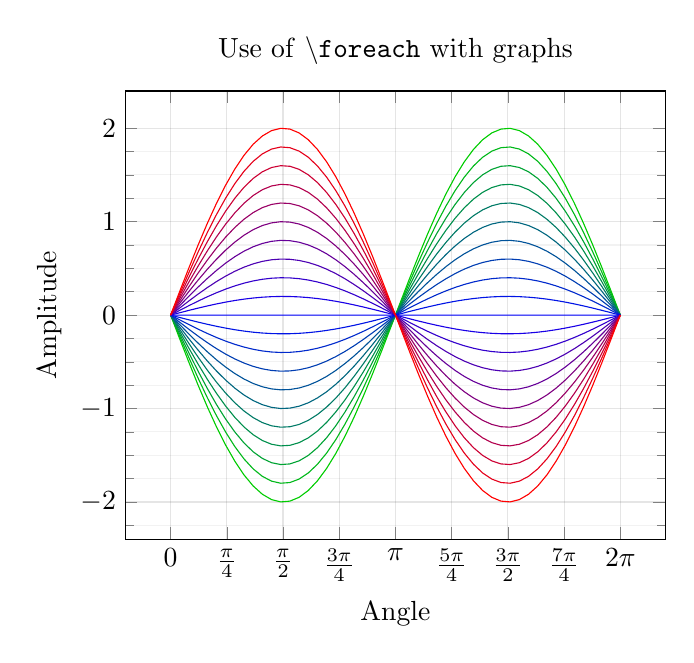
\begin{tikzpicture}
    \begin{axis}[
        	title = {Use of \texttt{\textbackslash foreach} with graphs},
            xlabel = Angle,
            ylabel = Amplitude,
            xtick = {0, 0.785398, ..., 6.5},
            xticklabels = {
                $0$,
                $\frac{\pi}{4}$,
                $\frac{\pi}{2}$,
                $\frac{3 \pi}{4}$,
                $\pi$,
                $\frac{5 \pi}{4}$,
                $\frac{3 \pi}{2}$,
                $\frac{7 \pi}{4}$,
                $2 \pi$
            }
        ]
        \foreach \i in {-2, -1.8, ..., 2.1} {
            % Calculate the hue mix
            \pgfmathparse{less(\i, 0) ? 100 - (\i + 2) / 2 * 100 : 0}
            \let\greenblue\pgfmathresult
            \pgfmathparse{less(\i, 0) ? 100 : 100 - (\i + 0) / 2 * 100}
            \let\bluered\pgfmathresult
            % Use \edef so that all the functions within are expanded at the
            % time of evaluation *except* for functions which are explicitly
            % told to no be expanded with \noexpand.
            \edef\temp{% 
                \noexpand\addplot[
                	black!20!green!\greenblue!blue!\bluered!red,
                	domain = 0:2*pi,
                    samples = 50,
                ] {\i * sin(x * 360 / (2 * pi))};
            }

            % Now \tmp contains what we would logically expect to be the
            % repeated code and we can print it out.
            \temp
        }
    \end{axis}
\end{tikzpicture}
\end{document}


%%% Local Variables: 
%%% TeX-master: t
%%% End: 
